\documentclass{article}
\usepackage[utf8]{inputenc}
\author{Kevin L}

\usepackage{amsmath,amsthm,amssymb,amsfonts,graphicx,framed,indentfirst}
\usepackage[normalem]{ulem}
\usepackage[italicdiff]{physics}
\usepackage[T1]{fontenc}
%\usepackage{pifont} %For unusual symbols
%\usepackage{mathdots} %For unusual combinations of dots
\usepackage{wrapfig}
\usepackage{lmodern,mathrsfs}
\usepackage[inline,shortlabels]{enumitem}
\setlist{topsep=2pt,itemsep=2pt,parsep=0pt,partopsep=0pt}
\usepackage[dvipsnames]{xcolor}
\usepackage[utf8]{inputenc}
\usepackage[a4paper, top=0.5in,bottom=0.2in, left=0.5in, right=0.5in, footskip=0.3in, includefoot]{geometry}
\usepackage[most]{tcolorbox}
\usepackage{tikz,tikz-3dplot,tikz-cd,tkz-tab,tkz-euclide,pgf,pgfplots}
\pgfplotsset{compat=newest}
\usepackage{multicol}
\usepackage[bottom,multiple]{footmisc} %ensures footnotes are at the bottom of the page, and separates footnotes by a comma if they are adjacent
% \usepackage[backend=bibtex,style=numeric]{biblatex}
% \renewcommand*{\finalnamedelim}{\addcomma\addspace} % forces authors' names to be separated by comma, instead of "and"
% \addbibresource{bibliography}
\usepackage{hyperref}
\usepackage[nameinlink]{cleveref} %nameinlink ensures that the entire element is clickable in the pdf, not just the number
\usetikzlibrary{positioning}
\newcommand{\ep}{\varepsilon}
\newcommand{\N}{\mathbb{N}}
\newcommand{\Q}{\mathbb{Q}}
\newcommand{\R}{\mathbb{R}}
\newcommand{\C}{\mathbb{C}}
\newcommand{\Z}{\mathbb{Z}}
\renewcommand{\iff}{\Leftrightarrow}
\newcommand{\dom}{\text{dom }}
\DeclareMathOperator{\range}{\text{range}}
\usepackage{mathtools}
\DeclarePairedDelimiter\ceil{\lceil}{\rceil}
\DeclarePairedDelimiter\floor{\lfloor}{\rfloor}

\newtheoremstyle{mystyle}{}{}{}{}{\sffamily\bfseries}{.}{ }{}
\newtheoremstyle{cstyle}{}{}{}{}{\sffamily\bfseries}{.}{ }{\thmnote{#3}}
\makeatletter
\renewenvironment{proof}[1][\proofname] {\par\pushQED{\qed}{\normalfont\sffamily\bfseries\topsep6\p@\@plus6\p@\relax #1\@addpunct{.} }}{\popQED\endtrivlist\@endpefalse}
\makeatother

\theoremstyle{mystyle}{\newtheorem{definition}{Definition}[section]}
\theoremstyle{mystyle}{\newtheorem{proposition}[definition]{Proposition}}
\theoremstyle{mystyle}{\newtheorem{theorem}[definition]{Theorem}}
\theoremstyle{mystyle}{\newtheorem{lemma}[definition]{Lemma}}
\theoremstyle{mystyle}{\newtheorem{corollary}[definition]{Corollary}}
\theoremstyle{mystyle}{\newtheorem*{remark}{Remark}}
\theoremstyle{mystyle}{\newtheorem*{remarks}{Remarks}}
\theoremstyle{mystyle}{\newtheorem*{example}{Example}}
\theoremstyle{mystyle}{\newtheorem*{examples}{Examples}}
\theoremstyle{definition}{\newtheorem*{exercise}{Exercise}}
\theoremstyle{cstyle}{\newtheorem*{cthm}{}}
\theoremstyle{cstyle}{\newtheorem*{clemma}{}}

\tcolorboxenvironment{definition}{boxrule=0pt,boxsep=0pt,colback={red!10},left=8pt,right=8pt,enhanced jigsaw, borderline west={2pt}{0pt}{red},sharp corners,before skip=10pt,after skip=10pt,breakable}
\tcolorboxenvironment{proposition}{boxrule=0pt,boxsep=0pt,colback={Orange!10},left=8pt,right=8pt,enhanced jigsaw, borderline west={2pt}{0pt}{Orange},sharp corners,before skip=10pt,after skip=10pt,breakable}
\tcolorboxenvironment{theorem}{boxrule=0pt,boxsep=0pt,colback={blue!10},left=8pt,right=8pt,enhanced jigsaw, borderline west={2pt}{0pt}{blue},sharp corners,before skip=10pt,after skip=10pt,breakable}
\tcolorboxenvironment{lemma}{boxrule=0pt,boxsep=0pt,colback={Cyan!10},left=8pt,right=8pt,enhanced jigsaw, borderline west={2pt}{0pt}{Cyan},sharp corners,before skip=10pt,after skip=10pt,breakable}
\tcolorboxenvironment{corollary}{boxrule=0pt,boxsep=0pt,colback={violet!10},left=8pt,right=8pt,enhanced jigsaw, borderline west={2pt}{0pt}{violet},sharp corners,before skip=10pt,after skip=10pt,breakable}
\tcolorboxenvironment{proof}{boxrule=0pt,boxsep=0pt,blanker,borderline west={2pt}{0pt}{CadetBlue!80!white},left=8pt,right=8pt,sharp corners,before skip=10pt,after skip=10pt,breakable}
\tcolorboxenvironment{remark}{boxrule=0pt,boxsep=0pt,blanker,borderline west={2pt}{0pt}{Green},left=8pt,right=8pt,before skip=10pt,after skip=10pt,breakable}
\tcolorboxenvironment{remarks}{boxrule=0pt,boxsep=0pt,blanker,borderline west={2pt}{0pt}{Green},left=8pt,right=8pt,before skip=10pt,after skip=10pt,breakable}
\tcolorboxenvironment{example}{boxrule=0pt,boxsep=0pt,blanker,borderline west={2pt}{0pt}{Black},left=8pt,right=8pt,sharp corners,before skip=10pt,after skip=10pt,breakable}
\tcolorboxenvironment{examples}{boxrule=0pt,boxsep=0pt,blanker,borderline west={2pt}{0pt}{Black},left=8pt,right=8pt,sharp corners,before skip=10pt,after skip=10pt,breakable}
\tcolorboxenvironment{cthm}{boxrule=0pt,boxsep=0pt,colback={blue!10},left=8pt,right=8pt,enhanced jigsaw, borderline west={2pt}{0pt}{blue},sharp corners,before skip=10pt,after skip=10pt,breakable}
\tcolorboxenvironment{clemma}{boxrule=0pt,boxsep=0pt,colback={Cyan!10},left=8pt,right=8pt,enhanced jigsaw, borderline west={2pt}{0pt}{Cyan},sharp corners,before skip=10pt,after skip=10pt,breakable}

\usepackage[explicit]{titlesec}
\titleformat{\section}{\fontsize{24}{30}\sffamily\bfseries}{\thesection}{20pt}{#1}
\titleformat{\subsection}{\fontsize{16}{18}\sffamily\bfseries}{\thesubsection}{12pt}{#1}
\titleformat{\subsubsection}{\fontsize{10}{12}\sffamily\large\bfseries}{\thesubsubsection}{8pt}{#1}

\titlespacing*{\section}{0pt}{5pt}{5pt}
\titlespacing*{\subsection}{0pt}{5pt}{5pt}
\titlespacing*{\subsubsection}{0pt}{5pt}{5pt}

\newcommand{\Disp}{\displaystyle}
\newcommand{\qe}{\hfill\(\bigtriangledown\)}
\DeclareMathAlphabet\mathbfcal{OMS}{cmsy}{b}{n}
\setlength{\parindent}{0.2in}
\setlength{\parskip}{0pt}
\setlength{\columnseprule}{0pt}

\definecolor{contcol1}{HTML}{72E094}
\definecolor{contcol2}{HTML}{24E2D6}
\definecolor{convcol1}{HTML}{C0392B}
\definecolor{convcol2}{HTML}{8E44AD}

\usepackage{setspace}
\setstretch{1.25}

\pgfplotsset{soldot/.style={color=black,only marks,mark=*},
  holdot/.style={color=black,fill=white,only marks,mark=*},
compat=1.12}

\counterwithin*{equation}{section}
\counterwithin*{equation}{subsection}

\renewcommand{\epsilon}{\varepsilon}

\usetikzlibrary{arrows}
\usetikzlibrary{shapes}
\usetikzlibrary{fit}
\begin{document}
\title{MATH 1800 Notes}
\date{Winter Term 1 2022}
\maketitle

\begin{tcolorbox}[title=, fonttitle=\huge\sffamily\bfseries\selectfont,interior style={left color=contcol1!40!white,right color=contcol2!40!white},frame style={left color=contcol1!80!white,right color=contcol2!80!white},coltitle=black,top=2mm,bottom=2mm,left=2mm,right=2mm,drop fuzzy shadow,enhanced,breakable]
  \tableofcontents
\end{tcolorbox}

\newpage
\section{Proofs}
\subsection{Proof by Induction}
\begin{definition}[The Principle of Mathematical Induction]
  Let $m$ be an integer, and let $P(n)$ be a statement for each integer $n \geq m$. If
  \begin{enumerate}
    \item $P(m)$ is true.
    \item the implication if $P(k)$, then $P(k+1)$ is true. $\forall \; k \in \Z > m$.
  \end{enumerate}
  $P(m)$ is called the \textbf{base case}, and $P(k+1)$ is called the \textbf{inductive step}.
\end{definition}
\begin{example}
  Prove $\forall \; n \in \N$, $1 + 2 + 3 + \ldots + n = \frac{n(n+1)}{2}$.
  Since $1 = \frac{1(2)}{2}$, the base case holds.
  Suppose $1 + 2 + 3 + \ldots + k = \frac{k(k+1)}{2}$ for any $k \in \N$. We must show that $1 + 2 + 3 + \ldots + k + (k+1)= \frac{(k+1)(k+2)}{2}$.\newline
  We have
  \begin{align*}
    1 + 2 + 3 + \ldots + k + (k+ 1) &= \frac{k(k+1)}{2} + (k + 1)\\
    &= (k+1)(\frac{k}{2}+1)\\
    &= (k+1)(\frac{k}{2}+\frac{2}{2})\\
    &= \frac{(k+1)(k+2)}{2}\\
  \end{align*}
  Thus by the principle of mathematical induction, it follows the result holds for all $n$.\qed
\end{example}
\begin{remark}
  There is an alternative proof to this problem discovered by Gauss.
  Let $S = 1 + 2 + \dots + (n-1) + n$.
  But $S = n + (n-1) + \dots + 2 + 1$.
  Adding these up, $2S = (n+1) + \dots + (n+1)$. Note that there are $n$ amount of terms.
  Then $S = \frac{n(n+1)}{2}$.
\end{remark}
\begin{example}
  Prove $\forall \; n \in \N$, $2^n > n$.
  Since $2^1 > 1$, the base case holds.
  Suppose $2^k > k \forall k \in \N$. Then we must show that $2^{k+1} > k+1$.
  We have
  \begin{align*}
    2^{k+1} &= 2 \cdot 2^k\\
    &> 2k\\
    &= k + k\\
    &\geq k + 1 \tag{k $\geq$ 1 from def.}\\
  \end{align*}
  \qed
\end{example}
\begin{remark}
  Note that the base case does not need to start at 1, as shown below.
\end{remark}
\begin{examples}
  \textbf{Example 1:}\newline
  Prove $\forall \; n \geq m \in \N$, $2^n \geq n^2$.
  Consider
  \begin{center}
    \begin{tabular}{ |c|c|c| }
      \hline
      $n$ & $2^n$ & $n^2$ \\
      \hline
      1 & 2 & 1 \\
      2 & 4 & 4 \\
      3 & 8 & 9 \\
      4 & 16 & 16 \\
      5 & 32 & 25 \\
      6 & 64 & 36 \\
      \hline
    \end{tabular}
  \end{center}
  It appears this holds for $n \geq 5$.

  Since $2^5 = 32 \geq 5^2 =25$, the base case holds.
  Suppose $2^k > k^2$, for some $k \in \Z$ with $k \geq 5$.
  We have
  \begin{align*}
    2^{k+1} &= 2^k \cdot 2^1\\
    &> 2k^2\\
    &= k^2 + k \cdot k\\
    &\geq k^2 + 5k \tag{$k \geq 5$}\\
    &= k^2 + 2k + 3k\\
    &\geq k^2 + 2k + 15 \tag{$k \geq 5$}\\
    &> k^2 + 2k + 1\\
    &= (k+1)^2\\
  \end{align*}
  \qed\newline
  \textbf{Example 2:}\newline
  Prove $3 \mid (2^{2n} - 1) \; \forall n \geq 0$.
  We proceed by induction.
  When $n = 0$, we have $2^{2 \cdot 0} - 1$, which is $0$, which is divisible by $3$.
  Suppose $3 \mid (2^{2k} - 1)$ for some $k \in \Z$. Thus,  $2^{2k} - 1 = 3c$ for some $c \in \Z$.
  Looking at $k+1$, we have
  \begin{align*}
    2^{2(k+1)}-1 &= 2^{2k+2} - 1\\
    &= 2^2 \cdot 2^{2k} -1\\
    &= 4(3c + 1) - 1\\
    &= 12c + 4 - 1\\
    &= 12c + 3\\
    &= 3(4c+1)\\
  \end{align*}
  Since $4c+1\in \Z$, $3 \mid 2^{2n}-1$.
  \qed\newline
  \textbf{Example 3:}\newline
  Let $n \in \N$. Then $1^2 + 2^2 + 3^2 + \dots + n^2 = \frac{n(n+1)(2n+1)}{6}$.
  We proceed by induction.
  Since $1^2 = 1 = \frac{(1)(2)(3)}{6}$, the base case holds.
  Suppose $1^2 + 2^2 + 3^2 + \dots + k^2 = \frac{k(k+1)(2k+1)}{6}$.
  We have
  \begin{align*}
    1^2 + 2^2 + 3^2 + \dots + k^2 + (k+1)^2 &= \frac{k(k+1)(2k+1)}{6} + (k+1)^2\\
    &= (k+1)\left(\frac{k(2k+1)}{6} + (k+1)\right)\\
    &= (k+1)\left(\frac{k(2k+1) + 6(k+1)}{6}\right)\\
    &= (k+1)\left(\frac{2k^2 + 7k + 6}{6}\right)\\
    &= (k+1)\left(\frac{(k+2)(2k+3)}{6}\right)\\
    &= \left(\frac{(k+1)(k+1+1)(2(k+1)+1)}{6}\right)\\
  \end{align*}
  \qed
\end{examples}
\begin{proposition}
  Recall that $n! = 1(2)(3)\ldots(n)$.
\end{proposition}
\begin{example}
  Let $n \in \N$. Then, $1 \cdot 1! + 2 \cdot 2! + \dots + n \cdot n! = (n+1)! - 1$.
  We proceed by induction.
  $1 \cdot 1! = 2! - 1 = 1$, so the base case holds.
  Suppose $1 \cdot 1! + 2 \cdot 2! + \dots + k \cdot k! = (k+1)! - 1$.
  Then,
  \begin{align*}
    1 \cdot 1! + 2 \cdot 2! + \dots + k \cdot k! + (k+1)\cdot (k+1)! &= (k+1)! - 1 + (k+1)(k+1)!.\\
    &=(k+1)! + (k+1)(k+1)! - 1\\
    &= (k+1)! (1 + (k+1)) - 1\\
    &= (k+1)! (k+2) - 1\\
    &= (k+2)! - 1\\
  \end{align*}\qed
\end{example}
\subsubsection{Proof by Strong Induction}
\begin{definition}
  [The Strong Principle of Mathematical Induction]
  Let $m$ be an integer, and let $P(n)$ be a statement for each integer $n \geq m$. If
  \begin{enumerate}
    \item P(m) is true
    \item the implication if $P(i)$ for every $i$ with $m \leq i \leq k$, then $P(k+1)$ is true for every integer $k \geq m$,
  \end{enumerate}
  Then $P(n)$ is true for every integer $n \geq m$.
  \newline
  In both regular and strong induction, the base case is the same, and in the inductive step we assume an inductive hypothesis and must prove the property holds for $k+1$.

  In regular induction, we get to assume the property holds for $k$. In strong induction, we get to assume the property holds for everything from the base case up to $k$.
\end{definition}
\begin{proposition}
  We can define a sequence by \textbf{recursion}.
\end{proposition}
\begin{example}
  Consider $a_1 = 1$, $a_2 = 4$, and $a_n = 2a_{n-1} -a_{a-2} + 2$ for $n \geq 3$. This is the sequence $(1, 4, 9, 16, 25, \ldots)$.
  Let us prove the general formula.
  Then, $a_n = n^2$ for all $n \in \N$.
  We proceed by strong induction. \newline
  Since $a_1 = 1 = 1^2$, the result holds for $n = 1$.\newline
  Let $k \in \N$ and suppose $a_i$ is $i^2$ for all $1 \leq i \leq k$.
  We must show that $a_{k+1} = (k+1)^2$. For $k \geq 2$, We have
  \begin{align*}
    a_{k+1} &=2a_k - a_{k-1} + 2\\
    &= 2k^2 - (k-1)^2 + 2 \tag{By our inductive hypothesis}\\
    &= 2k^2 - (k^2 - 2k + 1) + 2\\
    &= k^2 + 2k + 1\\
    &= (k+1)^2\\
  \end{align*}
  When $k = 1$, $a_{k+1} = a_2 = 4 = 2^2 = (k+1)^2$.
  \qed
\end{example}
\begin{proposition}
  The \textbf{Fibonacci Numbers} satisfy $F_1 = 1$, $F_2 = 1$, and $F_n = F_{n-1} + F_{n-2}$ for $n \geq 3$. The first few Fibonacci Numbers are $1, 1, 2, 4, 5, 6, 13, 21, 34, 55, 89$. This sequence has many interesting properties.
\end{proposition}
\begin{example}
  Let $m, n \geq 2$. Then, \[F_{m+n} = F_mF_{n-1} + F_{m+1}F_n\]
  Setting $m = n$, and then $m = n-1$ yields the formulas
  \[F_{2n} = F_n(F_{n-1} + F{n+1})\] and \[F_{2n-1} = F_{n-1}^2 + F_n^2\]

  Let $m, n \in N$ with $n \geq 2$. Then \[F_{m+n} = F_mF_{n-1} + F_{m+1}F_n\].

  Fix $m \in \N$. We proceed by induction on $n$. When $n = 2$,
  \begin{align*}
    F_mF_1 + F_{m+1}F_2 &= F_m + F_{m+1}\\
    &= F_{m+2}\\
  \end{align*}
  and so the base case holds.
  Let $k \in \N$ with $k \geq 2$ and suppose for $i$ with $2 \leq i \leq k$, we have \[F_m+i = F_mF_{i-1} + F_{m+1}F_i \]
  For $k \geq 3$, we have
  \begin{align*}
    F_{m + k + 1} &= F_{m + k} + F_{m + k - 1} \tag{By def. of fib}\\
    &= F_mF_{k-1} + F_{m+1}F_{k} + F_{m}F_{k-2} + F_{m+1}F_{k-1}\\
    &= F_m(F_{k-1} + F_{k-2}) + F_{m+1}(F_k + F_{k-1})\\
    &= F_mF_k + F_{m+1}F_{k+1}\tag{By def. of fib}\\
  \end{align*}
  When $k=2$,
  \begin{align*}
    F_mF_k + F_{m+1}F_{k+1} &= F_mF_2 + F_{m+1}F_3 \\
    &= F_m + 2F_{m+1}\\
    &= F_m + F_{m+1} + F_{m+1}\\
    &= F_{m+2} + F_{m+1}\\
    &= F_{m+3}\\
  \end{align*}
  \qed
\end{example}
\begin{remark}
  We will cover prove or disprove questions.
\end{remark}
\begin{examples}
  \textbf{Example 1:}\newline
  For $n \in \N$, $2^{(2^n)} \geq 4^{n!}$.
  Let's try some values.
  % insert table for n = 1, 2, 3
  This statement is false with $n=3$ yielding a counterexample.

  \textbf{Example 2:}\newline
  For every non-negative integer $n$, $5$ divides $2 \cdot 4^n + 3 \cdot 9^n$. Let's try some values.
  % insert table with n = 0, 1, 2, 3
  We think this may be true, so let us attempt a proof.
  We proceed by induction. When $n=0$, $2 \cdot 4^0 + 3 \cdot 9^0 = 5$, which is divisible by $5$. The base case holds.
  Let $k \in \N \cup \{0\}$ and suppose $5 \mid (2 \cdot 4^k + 3 \cdot 9^k)$. Then $2 \cdot 4^k + 3 \cdot 9^k = 5c$ for some $c \in \Z$. We have
  \begin{align*}
    2 \cdot 4^{k+1} + 3 \cdot 9^{k+1} &= 2 \cdot 4 \cdot 4^{k} + 3 \cdot 9 \cdot 9^{k}\\
    &= 2 \cdot 4 \cdot 4^k + 9(5c - 2 \cdot 4^k)\\
    &= 8 \cdot 4^k + 45c - 18 \cdot 4^k\\
    &= 45c - 10 \cdot 4^k\\
    &= 5(9c - 2 \cdot 4^k)\\
  \end{align*}
  Since $9c - 2 \cdot 4^k \in \Z$, $5 \mid 2 \cdot 4^n + 3 \cdot 9^n$. \qed\newline
  \textbf{Example 3:}\newline
  Every even integer $n \geq 4$ can be written as the sum of two primes.
  % insert table for n, p1 + p2 for some primes and n up to 22
  This is a famous problem called \textbf{Goldbach's Conjecture}, and this is still an open problem.
\end{examples}
\section{Relations}
\begin{remark}
  Recall a few theorems:
  Let $x, y, z \in \R$.
  \begin{itemize}
    \item If $x=y$ and $y=z$, then $x=z$.
    \item If $x < y$ and $y < z$, then $x < z$.
  \end{itemize}
  These different relations share the same property.
\end{remark}
\begin{definition}
  Let $A, B$ be sets. A \textbf{relation} $\mathrel{R}$ from $A$ to $B$ is a subset of the set
  \[
    \{(a, b) \mid a \in A \text{ and } b \in B \}
  \]
  which is equivalent to $A \times B$.

  Here, $(a, b)$ is an ordered pair.
  If $(a, b) \in \mathrel{R}$, we say that $a$ is related to $b$ by $\mathrel{R}$, and we write $a \mathrel{R} b$.
  If $(a, b) \not\in \mathrel{R}$, we say that $a$ is not related to $b$ by $\mathrel{R}$, and we write $a \not \mathrel{R} b$.

  Since $\emptyset$ is a subset of any set, it is always a relation from $A$ to $B$. For the relation $\emptyset$, no element of $A$ is related to any element of $B$.

  Since a set is always a subset of itself,
  \[
    \{(a, b) \mid a \in A \text{ and } b \in B\}
  \]
  is always a relation from $A$ to $B$. In this relation, each element of $A$ is related to every element of $B$.
\end{definition}

\begin{definition}
  Let $\mathrel{R}$ be a relation from $A$ to $B$. Then the \textbf{domain} of $\mathrel{R}$, denoted by $\dom{R}$ is the set
  \[
    \{a \in A \mid (a,b) \in \mathrel{R} \text{ for some $b \in B$}\}
  \]

  The \textbf{range} of $\mathrel{R}$, denoted by $\text{range}(\mathrel{R})$ is the set
  \[
    \{b \in B \mid (a,b) \in \mathrel{R} \text{ for some $a \in A$}\}
  \]
\end{definition}

\begin{definition}
  Let $\mathrel{R}$ be a relation from $A$ to $B$. The \textbf{inverse relation} of $\mathrel{R}$, denoted $\mathrel{R}^{-1}$, which is
  \[
    \{(b, a) \mid (a, b) \in \mathrel{R}\}
  \]
  It is a relation from $B$ to $A$.
\end{definition}
\begin{example}
  Let $A = \{a, b, c\}$ and $B = \{1, 2, 3\}$. Suppose $R = \{(a, 1), (a, 3), (b,2), (b, 3)$. Here, $b \mathrel{R} 2$, but $b \not \mathrel{R} 1$.

    The domain of $R$ is $\{a, b\}$, while the range is $\{1, 2, 3\}$.

    \[R^{-1} = \{(1, a), (3, a), (2, b), (3, b)\}\]
  \end{example}
  \begin{definition}
    A \textbf{relation on a set} $A$ is a relation from $A$ to $A$.
  \end{definition}
  \begin{examples}
    We define a relation on $\Z$:
    \[
      R = \{(a, b) \mid a, b \in \Z \text{ and } b = a+c \text{ for some } c \in \N\}
    \]
    We have for example, $2R4, 3R4, 4\not \mathrel{R}4, 5\not \mathrel{R}4$.

    In fact, this is the $<$ relation on $\Z$.

    We define a relation on $\Z$:
    \[
      R = \{(a, b) \mid a, b \in \Z \text{ and } 5 \mid (a-b)\}
    \]
    This is congruence modulo $5$ relation on $\Z$.
  \end{examples}
  \begin{definition}
    We define some properties of relations. Let $\mathrel{R}$ be a relation on a set $A$.

    \begin{enumerate}
      \item R is \textbf{reflexive} if $\forall x \in A$, $x \mathrel{R} x$.
      \item R is \textbf{symmetric} if $\forall x, y \in A$, $x \mathrel{R} y \implies y \mathrel{R} x$.
      \item R is \textbf{transitive} if $\forall x, y, z \in A$, if $(x \mathrel{R} y \wedge y \mathrel{R} z) \implies x \mathrel{R} z$.
    \end{enumerate}
  \end{definition}
  \begin{remark}
    Note for transitivity, $x, y, z$ do not have to be distinct. E.g, if $x \mathrel{R} y$ and $y \mathrel{R} x$, then $x \mathrel{R} x$. Furthermore, when manually checking we can ignore any elements of the form $(x, x)$ since they cannot lead to counterexamples. Also remember if $a \mathrel{R} b$ and $b \mathrel{R} a$, check for transitivity both ways, i.e. $a \mathrel{R} a$ and $b \mathrel{R} b$.
  \end{remark}
  \begin{examples}
    Let $A = \{1, 2, 3\}$. Consider
    \begin{align*}
      R_1 &= \{(a,b), (b, c), (c, b)\}\\
      R_2 &= \{(a, a), (a, b), (b, a), (b, b), (b, c), (c, b), (c, c)\}\\
      R_3 &= \{(a, a), (a, b), (b, a), (b, b), (c, c)\}\\
      R_4 &= \{(b, c)\}
    \end{align*}
    $R_1$ is not reflective since for example, $a \not \mathrel{R} a$.
    $R_1$ is not symmetric since for example, $a \mathrel{R} b \not \implies b \mathrel{R} a$.
    $R_1$ is not transitive since for example, $a \mathrel{R} b$ and $b \mathrel{R} c$ but $a \not \mathrel{R} c$.

    $R_2$ is reflective.
    $R_2$ is symmetric.
    $R_2$ is not transitive since for example, $a \mathrel{R} b$ and $b \mathrel{R} c$ but $a \not \mathrel{R} c$.

    $R_3$ is reflective.
    $R_3$ is symmetric.
    $R_3$ is transitive.

    $R_4$ is not reflective since for example, $a \not \mathrel{R} a$.
    $R_4$ is not symmetric since for example, $b \mathrel{R} c \not \implies c \mathrel{R} b$.
    $R_3$ is transitive (vacuously).
  \end{examples}
  \begin{definition}
    A relation on a set $A$ is called an \textbf{equivalence relation} if it is reflexive, symmetric, and transitive.

    The equality relation and $R_3$ above fulfill this criteria.
  \end{definition}
  \begin{definition}
    Let $R$ be an equivalence relation on $A$. For $a \in A$, the set
    \[
      [a] = \{x \in A \mid x \mathrel{R} a\}
    \]
    is called an \textbf{equivalence class}. It consists of all elements of $A$ that are related to $A$.
  \end{definition}
  \begin{examples}
    Fix a number $n \in \N$, with $n\geq 2$ and consider the congruence modulo $n$ relation on $\Z$.
    Since
    \begin{align*}
      x &\equiv x \pmod{n}\\
      x &\equiv y \implies y \equiv x\\
      x &\equiv y \wedge y \equiv z \implies x \equiv z\\
    \end{align*}
    The congruence relation is an equivalence class.

    \textbf{Example 2:}

    Let $A = \{a, b, c\}$ and $R = \{(a, a), (a, b), (b, a), (b, a), (c, c)\}$
    Then
    \begin{align*}
      [a] &= \{a, b\}\\
      [b] &= \{a, b\}\\
      [c] &= \{c\}\\
    \end{align*}

    \textbf{Example 3:}

    Let $A = \{1, 2, 3\}$ and $R = \{(a, a), (a, b), (b, a), (b, a), (c, c)\}$
    It can be shown $R$ is an equivalence relation.
    Then,
    \begin{align*}
      [1] &= \{1, 3, 6\}\\
      [2] &= \{2, 4\}\\
      [3] &= \{1, 3, 6\}\\
      [4] &= \{2, 4\}\\
      [5] &= \{5\}\\
      [6] &= \{1, 3, 6\}\\
    \end{align*}

    \textbf{Example 4:}

    Consider the equality relation on $\Z$. Let $a \in \Z$, then
    \begin{align*}
      [a] &= \{x \in \Z \mid x \mathrel{R} a\}\\
      &= \{x \in \Z \mid x = a\}\\
      &= \{a\}
    \end{align*}
    \textbf{Example 5:}

    Define $R$ on $Z$ by $a \mathrel{R} b$ iff $|a| = |b|$. One may show this is a equivalence relation. Then,
    \[
      [a] = \{x \in \Z \mid x \mathrel{R} a \} = \{x \in \Z \mid |x| = |a|\} = \{a, -a\}
    \]

    \textbf{Example 6:}

    Define $R$ on $Z$ by $a \mathrel{R} b$ if $5a+b$ is even.
    Then $R$ is an equivalence relation.

    We first show $R$ us reflexive.
    Let $a \in \Z$, then $5a + a = 6a = 2 \cdot 3a$. Since $3a \in \Z$, $5a + a$ is even and so $R$ is reflexive.

    Now we show $R$ is symmetric.
    Suppose $a \mathrel{R} b$, then $5a + b = 2k$ for some $k \in \Z$.
    We have
    \begin{align*}
      5b + a &= 5(2k - 5a) + a\\
      &= 10k - 25a + a\\
      &= 10k - 24a\\
      &= 2(5k-12a)\\
    \end{align*}
    Thus, $b \mathrel{R} a$.

    We now show $R$ is transitive.
    Suppose $a \mathrel{R} b$ and $b \mathrel{R} c$.
    Then, $5a + b = 2k$ and $5b + c = 2l$ for some $k, l \in \Z$.
    We have
    \begin{align*}
      5a + c &= 2k-b + 2l - 5b\\
      &= 2k + 2l - 6b\\
      &= 2(k+l-3b)
    \end{align*}
    Since the above is an integer, $5a + c$ is even and so $R$ is transitive.

    Let's look at the equivalence classes. First, we check for 1 specific element.
    \[
      [0] = \{x \in \Z \mid x \mathrel{R} 0\} = \{x \in \Z \mid 5x \text{ is even}\} = \{x \in \Z \mid x \text{ is even}\}
    \]

    Let $a = 2k$. Then,
    \begin{align*}
      [a] &= \{x \in \Z \mid x \mathrel{R} a\}\\
      &= \{x \in \Z \mid 5x + a \text{ is even}\}\\
      &= \{x\in \Z \mid x \text{ is even}\}
    \end{align*}
    Let $b = 2l + 1$. Then,
    \begin{align*}
      b &= \{x\in \Z \mid 5x + b \text{ is even}\}\\
      &= \{x \in \Z \mid x \text{ is odd}\}\\
    \end{align*}
    Thus, there are 2 distinct classes
    \[
      [0] = [2] = [4] = \dots
    \]
    and \[
      [1] = [3] = [5] = \dots
    \]
  \end{examples}
  \begin{theorem}
    Let $R$ be an equivalence relation on a non-empty set $A$. Let $a, b \in A$. Then \[
      [a] = [b] \iff a \mathrel{R} b
    \]
  \end{theorem}
  \begin{proof}

    We prove the forwards direction.
    Suppose $[a] = [b]$. Then as $R$ is reflective we have $a \mathrel{R} a$, and so $a \in [a]$ and since $[a] = [b]$, we have $a \in [B]$. Thus, $a \mathrel{R} b$.

    We prove the reverse direction.
    Suppose $a \mathrel{R} b$. We show $[a] \subseteq [b]$. Let $x \in [a]$, then $x \mathrel{R} a$. Then $x \mathrel{R} a$ and $a \mathrel{R} b$, and as $\mathrel{R}$ is transitive, we have $x \mathrel{R} b$ and so $[a] \subseteq [b]$.

    Now we show $[b] \subseteq [a]$. Let $x \in [b]$, then $x \mathrel{R} b$. As $a \mathrel{R} b$, and $\mathrel{R}$ is symmetric, we have $b \mathrel{R} a$. We have $x \mathrel{R} b$ and $b \mathrel{R} a$, and as $R$ is transitive, we have $x \mathrel{R} a$. Thus, $[b] \subseteq [a]$.

    Thus $[a] = [b]$.
  \end{proof}
  \begin{theorem}
    Let $R$ be a equivalence relation on a non-empty set $A$. Then each element belongs to $1$ equivalence class.
  \end{theorem}
  \begin{proof}
    Let $a \in A$. As $R$ is reflective, we have $a \mathrel{R} a$, so $a \in [A]$. We must now show uniqueness.
    Suppose $a \mathrel{R} b$. By previous theorem, $[b] = [a]$, and thus $a$ belongs to 1 unique equivalence class.
  \end{proof}
  \begin{proposition}
    Equivalence classes of $\mathrel{R}$ form a partition of $A$.
    \begin{itemize}
      \item They are non-empty.
      \item They are disjoint.
      \item They have a union of $A$.
    \end{itemize}
  \end{proposition}
  \begin{example}
    We know that congruence mod $n$ is an equivalence relation. What are the equivalence classes? We work with mod $3$ for now.

    \[
      [0] = \{x \in \Z \mid x \mathrel{R} 0\} = \{x \in \Z \mid x \equiv 0 \pmod{3}\} = \{x \in \Z \mid 3 \mid x\} = \{3k \mid k \in \Z\}
    \]
    \[
      [1] = \{x \in \Z \mid x \mathrel{R} 1\} = \{x \in \Z \mid x \equiv 1 \pmod{3}\} = \{x \in \Z \mid 3 \mid (x-1)\} = \{3k + 1 \mid k \in \Z\}
    \]
    \[
      [2] = \{x \in \Z \mid x \mathrel{R} 2\} = \{x \in \Z \mid x \equiv 2 \pmod{3}\} = \{x \in \Z \mid 3 \mid (x-2)\} = \{3k + 2 \mid k \in \Z\}
    \]
    The union of these classes is $\Z$.
    In general, there are $n$ equivalence classes for the relation congruence mod $n$.
  \end{example}
  \begin{proposition}
    \[\Z_n = \{[0], [1], \ldots, [n-1]\}\]

    These are called the integers modulo $n$, and the elements are called \textbf{residue classes}.
  \end{proposition}
  \begin{definition}
    Let $[a]$ and $[b]$ be two residue classes in $\Z_n$. We define
    \[
      [a] + [b] = [a+b]
    \]
    \[
      [a][b] = [ab]
    \]
  \end{definition}
  \begin{example}
    We have (working in $\Z_7$)
    \[
      [6] + [3] = [6+3] = [9] = [7]
    \]
    and
    \[
      [6][3] = [6 \times 3] = [18]
    \]
  \end{example}
  \begin{remark}
    There is a potential problem. An equivalence class modulo $n$ has an infinite number of representatives, but our operation seems to depend on which ones are being used.
  \end{remark}
  \begin{theorem}
    Let $n \in \N$, $n \geq 2$. Then $+$, $\times$ on $\Z_n$ are well defined.
    That is, if $[a] = [b]$ and $[c] = [d]$, then $[a+c]=[b+d]$ and $[ac] = [bd]$.
  \end{theorem}
  \begin{proof}
    Suppose $[a] = [b]$ and $[c] = [d]$. Then $a \equiv b \pmod{n}$ and $c \equiv d \pmod{n}$. Thus $n \mid (a-b)$ and $n \mid (c-d)$. Thus $a-b = nk$ ($a = nk + b$) and $c-d = nl$ ($c = nl + d$) for some $k, l \in \Z$.
    We have
    \begin{align*}
      a+c - (b+d) &= a - b + c - d\\
      &= nk - nl\\
      &= n(k-l)\\
    \end{align*}
    Since $k - l \in \Z$, we have $n \mid ((a+c) - (b+d))$, thus $a + c \equiv b + d \pmod{n}$ and so $[a+b] = [c+d]$.

    We also have
    \begin{align*}
      ac - bd &= (b + nk)c - b(c - nl)\\
      &= n(kc + bl)\\
    \end{align*}
    So by the same argument $[ac] = [bd]$.
  \end{proof}
  \begin{definition}
    Let $k \in \N$, $a \in \Z$. Then
    \[
      [a^k] = [a\cdot a \cdot a \dots] \text{ ($k$ times) } = [a]^k
    \]
  \end{definition}
  \begin{example}
    Show that for $n \in \N$, $5$ divides $2 \cdot 4^n + 3 \cdot 9^n$.
    We have
    \begin{align*}
      [2 \cdot 4^n + 3 \cdot 9^n] &=  [2 \cdot 4^n] + [3 \cdot 9^n]\\
      &= [2 \cdot 4^n] + [3][9^n]\\
      &= [2 \cdot 4^n] + [3][9]^n\\
      &= [2 \cdot 4^n] + [3][4]^n\\
      &= [2 \cdot 4^n] + [3][4^n]\\
      &= [2 \cdot 4^n] + [3 \cdot 4^n]\\
      &= [2 \cdot 4^n + 3 \cdot 4^n]\\
      &= [5 \cdot 4^n]\\
      &= [5][4^n]\\
      &= [0][4^n]\\
      &= [0 \cdot 4^n]\\
      &= [0]\\
    \end{align*}
    Thus for any $n \in \N$, $2 \cdot 4^n + 3 \cdot 9^n \equiv 0 \pmod{5}$.

    We can drop the square brackets and just write $\pmod{5}$.
    \begin{align*}
      2 \cdot 4n + 3 \cdot 9n &\equiv 2 \cdot 4n + 3 \cdot 4n \pmod{5}\\
      &\equiv 5 \cdot 4n \pmod{5}\\
      &\equiv 0 \cdot 4n \pmod{5}\\
      &\equiv 0 \pmod{5}\\
    \end{align*}
  \end{example}
  \begin{proposition}
    Let $n \in \N$. Then $9 \mid n$ iff $9$ divides the digits of $n$.
  \end{proposition}
  \begin{proof}
    Let $d_k, d_{k-1}, \ldots, d_1, d_0$ be the digits of $n$.
    \[
      n = d_k10^k + d_{k-1}10^{k-1} + \dots + d_110^1 +d_0
    \]
    \begin{align*}
      n &\equiv d_k1^k + d_{k-1}1^{k-1} + \dots + d_1 + d_0 \pmod{9}\\
      &\equiv d_k + d_{k-1} + \dots + d_1 + d_0
    \end{align*}
    This is because $10 \equiv 1 \pmod{9}$.

    Suppose $9 \mid n$, then $n \equiv 0 \pmod{9}$, so by the above the digits must be equivalent to $0$.
    Thus $9 \mid (d_k + d_{k-1} + \dots + d_1 + d_0)$.

    Now suppose $9 \mid (d_k + d_{k-1} + \dots + d_1 + d_0)$. Then by above $n \equiv 0 \pmod{9}$, and thus $9 \mid n$.
  \end{proof}
  \subsection{Functions}
  \begin{definition}
    Let $A$ and $B$ be non-empty sets. A \textbf{function} f from $A$ to $B$, written $f: A\to B$ is a relation from $A$ to $B$ where every element of $A$ is the first co-ordinate of exactly one ordered pair in $f$.
  \end{definition}
  \begin{definition}
    Here, $\dom{f} = A$
  \end{definition}
  \begin{definition}
    B is called the \textbf{co-domain} of $f$.
  \end{definition}
  \begin{definition}
    If $(a, b) \in f$, we write $f(a) = b$.
  \end{definition}
  \begin{definition}
    $b$ is called the \textbf{image} of $a$, and we say that $f$ \textbf{maps} $a$ to $b$.
  \end{definition}
  \begin{definition}
    The \textbf{range} of $f$ is
    \begin{align*}
      \range{f} &= \{b \in B \mid (a, b) \in f \text{ for some }a \in A\}\\
      &= \{f(a) \mid a \in A\}
    \end{align*}
  \end{definition}
  \begin{example}
    Let $A = \{a, b, c\}$ and $B = \{1, 2, 3, 4\}$.
    Which of the following are functions?

    \begin{align*}
      f_1 &= \{(a, 1), (b, 4), (c, 4)\}\\
      f_2 &= \{(a, 2), (a, 3), (b, 4), (c, 1)\}\\
      f_3 &= \{(a, 1), (b, 2)\}
    \end{align*}
    Of above, only $f_1$ is a function.

    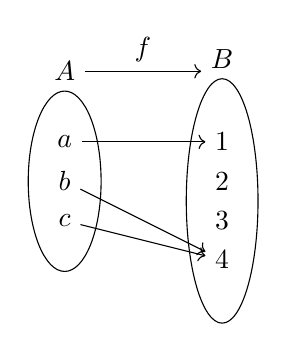
\begin{tikzpicture}
      \foreach[count=\i] \lseti/\lsetmi in {A/{$a$,$b$,$c$},B/{1,2,3,4}} {
        \begin{scope}[local bounding box=\lseti, x=2cm, y=0.5cm]
          \foreach[count=\j] \lj in \lsetmi {
            \node[minimum width=1em] (n-\j-\lseti) at (\i,-\j) {\lj};
          }
        \end{scope}
        \node[ellipse, draw, fit=(\lseti),
        label={[name=l-\lseti]above:$\lseti$}] {};
      }
      \draw[->] (n-1-A) -- (n-1-B);
      \draw[->] (n-2-A) -- (n-4-B);
      \draw[->] (n-3-A) -- (n-4-B);
      \draw[->] (l-A) -- node[above]{$f$}(l-A.center-|l-B.west);
    \end{tikzpicture}
    The range of $f$ is $\{1, 4\}$.
  \end{example}
  \begin{definition}
    We say two functions $f:A\to B$ and $g: A \to B$ are \textbf{equal}, written $f = g$ if for all $a \in A$, $f(a) = g(a)$. This implies that $f$ and $g$ are equal as relations.
  \end{definition}
  \begin{example}
    Let $f = \{(x, x^2\mid x \in \R\}$ is a function from $\R$ to $\R$. Here, for any $x \in \R$, we have $f(x) = x^2$.

      Note that the function $f$ is the set of ordered pairs, while $f(x) = x^2$ is the rule that describes the image of an arbitrary $x \in \R$.
    \end{example}
    \begin{definition}
      Let $f: A \to B$ be a function, and let $C \subseteq A$. The image of $C$ is the set
      \[
        f(C) = \{f(x) \mid x \in C\}
      \]
      We have $f(C) \subseteq B$.
      Note that $f(A) = \range{f}$.
    \end{definition}
    \begin{definition}
      Let $D \subseteq B$. The \textbf{inverse image} or \textbf{preimage} of $D$ is the set
      \[
        f^{-1}(D) = \{a \in A \mid f(a) \in D\}
      \]
    \end{definition}
    \begin{example}
      Let $A = \{a, b, c, d, e\}$ and $B = \{1, \dots, 6\}$.
      Let $f = \{(a, 5), (b, 2), (c, 3), (d, 5), (e, 6)\}$.

      Let $c_1 = \{c, d, e\}, c_2 = \{a, d\},$ and $c_3 = \{b\}$.

      \begin{align*}
        f(c_1) &= \{3, 5, 6\}\\
        f(c_2) &= \{5\}\\
        f(c_3) &= \{2\}\\
        f(A) &= \{2, 3, 5, 6\}\\
        \\
        f^{-1}(\{3, 5, 6\}) &= \{a, c, d, e\}\\
        f^{-1}(\{5\}) &= \{a, d\}\\
        f^{-1}(\{1\}) &= \emptyset\\
        f^{-1}(B) &= A\\
      \end{align*}
    \end{example}
    \begin{example}
      Let $f: \Q \to \Q$ be defined by $f(r) = \frac{3r}{2}$. Let $E$ be the set of even integers.

      \begin{align*}
        f(\Z) &= \{f(n) \mid n \in \Z\}\\
        &= \{\frac{3n}{2} \mid n \in \Z\}\\
        \\
        f(E) &= \{f(n) \mid n \in E\}\\
        &= \{f(2k) \mid k \in \Z\}\\
        &= \{3k \mid k \in \Z\}\\
        \\
        f^{-1}(\Z) &= \{r \in \Q \mid f(r) \in \Z\}\\
        &= \{r \in \Q \mid \frac{3r}{2} \in \Z\}\\
        &= \{\frac{2n}{3} \mid n \in \Z\}\\
        \\
        f^{-1}(E) &= \{r \in \Q \mid f(r) \in E\}\\
        &= \{ r\in \Q \mid \frac{3r}{2} \in E\}\\
        &= \{\frac{4k}{3} \mid k \in \Z\}\\
      \end{align*}
    \end{example}
    \begin{definition}
      Let $A$ and $B$ be non-empty sets. Then $B^A$ is the set of all functions from $A$ to $B$.

      In general, if $A, B$ are finite, then $|B^A| = |B|^{|A|}$.
    \end{definition}
    \begin{example}
      Let $A = \{a, b, c\}$ and $B = \{x, y\}$.
      \begin{align*}
        f_1 &= \{(a, x), (b, x), (c, x)\}\\
        f_2 &= \{(a, x), (b, x), (c, y)\}\\
        f_3 &= \{(a, x), (b, y), (c, x)\}\\
        f_4 &= \{(a, y), (b, x), (c, x)\}\\
        f_5 &= \{(a, x), (b, y), (c, y)\}\\
        f_6 &= \{(a, y), (b, y), (c, x)\}\\
        f_7 &= \{(a, y), (b, x), (c, y)\}\\
        f_8 &= \{(a, y), (b, y), (c, y)\}\\
        \\
        B^A &= \{f_1, \dots, f_8\}\\
      \end{align*}
    \end{example}
    \subsubsection{Properties of Functions}
    \begin{definition}
      A function $f: A \to B$ is \textbf{injective} or \textbf{one-to-one} if $\forall x, y \in A$,
      \[
        x \neq y \implies f(x) \neq f(y)
      \] and
      \[
        f(x) = f(y) \implies x = y
      \]
      If $A$ and $B$ are finite, and $f$ is injective, then $|A| \leq |B|$.
    \end{definition}
    \begin{example}
      Prove that $f(x) = x^2 + x + 1$ is not injective.

      Let $x, y \in \R$ and suppose $f(x) = f(y)$. Then
      \begin{align*}
        x^2 + x + 1 &= y^2 + y + 1\\
        0 &= x^2 - y^2 + x - y\\
        &= (x-y)(x+y) + (x-y)\\
        &= (x-y)(x+y+1)
      \end{align*}
      This is satisfied when $x = y$ or when $x + y + 1 = 0$. Thus $f(x) = f(y)$ does not imply $x = 0$ as there is another possibility.
    \end{example}
    \begin{definition}
      A function $f: A \to B$ is \textbf{surjective} or \textbf{onto} if for each $y \in B$, there exists $x \in A$ with $f(x) = y$. Equivalently, $f$ is surjective if $\range{f} = B$. That is $f(A) = B$.

      If $A$ and $B$ are finite sets and $f$ is surjective, then $|A| \geq |B|$.
    \end{definition}
    \begin{example}
      Show that $f : \R \to \R$ defined by $f(x) = 7x + 5$ is surjective.

      Rough:
      Given $y \in \R$, show that $\exists x \in \R$ s.t. $f(x)=y$. That is, $7x+ 5 = y \iff x = \frac{y-5}{7}$.

      Proof:
      Let $y \in \R$, and let $x = \frac{y-5}{7}$. Then $f(x) = y$.
    \end{example}
    \begin{example}
      Show that $f : \Z \to \Z$ defined by $f(x) = 7x + 5$ is not surjective.

      Since $0 \in \Z$, but $\not\exists x \in \Z$ s.t. $f(x) = 0$, $f$ is not surjective. (We need $x = \frac{-5}{7}$)
    \end{example}
    \begin{definition}
      A function $f: A \to B$ is \textbf{bijective} if it is injective and surjective.

      If $A$ and $B$ are finite sets and $f$ is bijective, then $|A| = |B|$.
    \end{definition}
    \begin{remark}
      Injective means everything gets “hit” at most once.

      Surjective means everything gets “hit” at least once.

      Bijective means everything gets “hit” exactly once.

      A bijective function from A to B is a perfect pairing of the elements of A with the elements of B.
    \end{remark}
    \begin{example}
      Show that $f : \R - \{-1\} \to \R - \{1\}$ is bijective.

      We show $f$ is injective. Suppose $f(x) = f(y)$, for $x, y \in \dom{f}$.

      Then
      \begin{flalign*}
        \frac{x-1}{x+1} &= \frac{y-1}{y+1}\\
        \implies (x-1)(y+1) &= (y-1)(x+1)\\
        \implies xy + x - y - 1 &= xy + y - x - 1\\
        \implies x - y &= y - x\\
        \implies 2x &= 2y\\
        \implies x &= y
      \end{flalign*}

      Rough Work:
      Given $y \in \R - \{1\}$, we find $x \in \dom{f}$ with $f(x) = y$.

      \begin{flalign*}
        \frac{x-1}{x+1} &= y\\
        \iff x-1 &= y(x+1)\\
        \iff x-1 &= yx + y\\
        \iff x - yx &= y + 1\\
        \iff x(1-y) &= y+1\\
        \iff x &= \frac{y+1}{1-y}
      \end{flalign*}

      Proof:
      We show $f$ is surjective. Let $y \in \R - \{1\}$. Then take $x = \frac{y+1}{1-y}$. $f(x) = y$.
    \end{example}
    \begin{definition}
      Let $A$ be nonempty set. The function $i_A: A \to A$ defined by $i_A(a) = a$ for all $a \in A$ is called the \textbf{identity function} on $A$.
    \end{definition}
    \begin{definition}
      Let $A, B, C$ be non-empty sets, and let $f: A \to B$ and $g: B \to C$ be functions. The composition $g \circ f$ is the function from $A \to C$ defined by
      \[
        (g \circ f)(x) = g(f(x))
      \]
      for all $x \in A$.
    \end{definition}
    \begin{example}
      Let
      \begin{align*}
        A &= \{1, 2, 3, 4\}\\
        B &= \{a, b, c, d\}\\
        C &= \{x, y, z\}\\
      \end{align*}
      We define $f: A \to B$ and $g: B \to C$ as
      \begin{align*}
        f &= \{(1, c), (2, b), (3, a), (4, a)\}\\
        g &= \{(a, x), (b, z), (c, x), (d, y)\}\\
      \end{align*}
      Then $g \circ f = \{(1, x), (2, z), (3, x), (4, x)\}$.
    \end{example}
    \begin{example}
      Let $f: \Z \to \Z$ and $g: \Z \to \Z$ be defined by $f(n) = 2n + 1$ and $g(n) = n^2 - 1$.

      Then $g \circ f = (2n+1)^2 - 1$ and $f \circ g = 2(n^2-1) + 1$.
    \end{example}
    \begin{theorem}
      Let $f: A \to B$ and $g: B \to C$. Then
      \begin{itemize}
        \item If $f, g$ are injective, then $f \circ g$ is injective.
        \item If $f, g$ are surjective, then $f \circ g$ is surjective.
      \end{itemize}
    \end{theorem}
    \begin{proof}
      Let $f, g$ be injective. Suppose $(g \circ f)(x) = (g \circ f)(y)$. Then
      \begin{align*}
        (g \circ f)(x) &= (g \circ f)(y)\\
        \implies g(f(x)) &= g(f(y))\\
        \implies f(x) &= f(y)\\
        \implies x &= y\\
      \end{align*}
      Thus $f \circ g$ is injective.

      Let $f, g$ be surjective. Let $c \in C$. Since $g$ is surjective, we have $b \in B$ with $g(b) =C$. Since $f$ is surjective, we have $a \in A$ where $f(a)  =b$. We have
      \begin{align*}
        (g \circ f)(a) &= g(f(a))\\
        &= f(b)\\
        &= c\\
      \end{align*}
    \end{proof}
    \begin{theorem}
      Let $f: A \to B$ be a function. The inverse relation $f^{-1}: B \to A$ is a function iff $f$ is bijective. Furthermore, if $f$ is bijective, so is $f^{-1}$.
    \end{theorem}
    \begin{proof}
      We prove the forwards direction.
      Suppose $f^{-1}$ is a function from $B$ to $A$. We show that $f$ is bijective.

      Suppose $f(x_1) = f(x_2) = y$ where $x_1, x_2 \in A$ and $y \in B$.
      Then, $(x_1, y), (x_2, y) \in f$ and so $(y, x_1), (y, x_2) \in f^{-1}$. Since $f^{-1}$ is a function, $x_1 = x_2$.
      Thus $f$ is injective.

      Now let $y \in B$. Since $f^{-1}$ is a function from $B$ to $A$, there is some $x \in A$ with $f^{-1}(y) = x$. That is, $(y, x) \in f^{-1}$, and so $(x, y) \in f$. Hence $f(x) = y$. Thus $f$ is surjective,

      As $f$ is injective and surjective, it is bijective.

      Now we prove the reverse direction.

      Suppose $f$ is bijective. We will show $f^{-1}$ is a function.

      Let $b \in B$. Since $f$ is surjective, there is an $a \in A$ such that $f(a) = b$. Then $(a, b) \in f$ and so $(b, a) \in f^{-1}$. We must show that $(b, a)$ is the unique element with first element $b$. Suppose $(b, a), (b, a') \in f^{-1}$. Then $(a, b) \in f$ and $(a', b) \in f$. Since $f$ is injective, $a' = a$. Thus $\forall b \in B, \exists! a$ with $(b, a) \in f^{-1}$. Thus $f^{-1}$ is a function.

      Finally, we show that if $f$ is bijective, so is $f^{-1}$.

      Suppose $f^{-1}(x_1) = f^{-1}(x_2) = y$ for $x_1, x_2 \in B$ and $y \in A$. The ordered pairs
      \begin{align*}
        (x_1, y), (x_2, y) \in f^{-1} &\implies (y, x_1), (y, x_2) \in f\\
        &\implies x_1 = x_2
      \end{align*}
      since $f$ is a function. Thus $f^{-1}$ is injective.

      Let $a \in A$ and let $f(a) = b$. Then $(a, b) \in f \implies (b, a) \in f^{-1}$. Since $f^{-1}$ is a function, $f^{-1}(b) = a$. Thus $f^{-1}$ is surjective. As $f^{-1}$ is injective and surjective, it is bijective.
    \end{proof}
    \begin{theorem}
      If $f: A \to B$ and $g: B \to A$ are functions satisfying $g \circ f = i_A$ and $f \circ g = i_B$, then $f, g$ are bijective with $g = f^{-1}$.
    \end{theorem}
    \begin{proof}
      Let $f: A \to B$ and $g: B \to A$.
      Let $a \in A$ and suppose $f(a) = b$. Then $(a, b) \in f$, and so $(b, a) \in f^{-1}$. Thus $f^{-1}(b) = a$.

      We have \[
        (f^{-1} \circ f)(a) = f^{-1}(f(a)) = f^{-1}(b) = a
      \] and \[
        (f \circ f^{-1})(b) = f(f^{-1}(b)) = f(a) = b
      \]
    \end{proof}
    \begin{example}
      We saw $f: \R - \{-1\} \to \R - \{1\}$ defined by $f(x) = \frac{x-1}{x+1}$ is bijective. Let's find a formula for $f^{-1}$.

      We use the fact that $(f \circ f^{-1})(x) = x$.

      Thus,
      \begin{align*}
        x &= f(f^{-1}(x))\\
        &= \frac{ff^{-1}(x) - 1}{f^{-1}(x) + 1}\\
        \implies xf^{-1}(x) + x &= f^{-1}(x) - 1\\
        \implies xf^{-1}(x) - f^{-1}(x) &= -1 - x\\
        \implies f^{-1}(x)(x-1) &= -1 - x\\
        \implies f^{-1}(x) &= \frac{1+x}{1-x}\\
      \end{align*}
    \end{example}
    \begin{remark}
      In general, $f^{-1}(x) \neq \frac{1}{f(x)}$.
    \end{remark}
    \begin{remark}
      It's not always possible to solve for the formula of an inverse function algebraically. For example,

      One may show that the function $e^x$ is bijective. We call the inverse $\ln x$.

      One may show that the function $\sin x$ is bijective (on an interval). We call the inverse $\arcsin x$.

      One may show that the function $f(x) = 3x^7 + 5x^3 + 4x - 1$ is bijective. There is no way to write a formula for the inverse. As a set, it is
      \[
        f^{-1} = \{(3x^7 + 5x^3 + 4x - 1, x) \mid x \in \R\}
      \]
    \end{remark}
    \section{Counting Arguments}
    \begin{definition}
      The \textbf{Principle of Inclusion/Exclusion} states, if $A_1, A_2, A_3$ are finite sets, then:
      \[
        |A_1 \cup A_2| = |A_1| + |A_2| - |A_1 \cap A_2|
      \]

      Note that if $A_1, A_2, \ldots, A_n$ are mutually disjoint, then \[
        |A_1 \cup A_2 \cup dots \cup A_n| = |A_1| + |A_2| + \dots + |A_n|
      \]
      This is called \textbf{sum rule}
    \end{definition}
    \begin{definition}
      Suppose a procedure can be broken down into a sequence of 2 tasks, and for each of the $n_1$ ways to do the first task, there are $n_2$ ways to do the second. Then there are $n_1n_2$ ways to do the procedure. This is the \textbf{product rule}.
    \end{definition}
    \begin{example}
      How many 2 letter initials are there?

      26 choices for first, 26 for second.
      Total is $26 \times 26$.

      How many non-repeating?
      Total is $26 \times 25$.
    \end{example}
    \begin{example}
      If $A = \{x_1, \ldots, x_m\}$ and $B$ are finite sets with $|A| = m$ and $|B| = n$, how many functions are there that map from $A$ to $B$?

      Assign values to $f(x)$ for each of the elements of $A$.

      For $x_1$, there are $n$ choices.
      For $x_2$, there are $n$ choices and so on.

      Thus we have $n \cdot n \cdot n \cdot \dots = n^m = |B|^|{A|}$

      How many injective functions?
      For $x_1$, there are $n$ choices.
      For $x_2$, there are $n-1$ choices and so on.

      Thus we have $n(n-1)\ldots(n-(m-1)) = \frac{n!}{(n-m)!}$
    \end{example}
    \begin{cthm}[The Pigeonhole Principle]
      Let $k \in \N$. If $k+1$ or more objects are placed into $k$ boxes, then at least one box contains two or more objects.
    \end{cthm}
    \begin{proof}
      Suppose not. Then each of the $k$ boxes contains at most one object, giving at most $k$ objects. A contradiction.
    \end{proof}
    \begin{example}
      Let $f: A \to B$ be a function with $|A| \geq k+1$ and $|B| = k$. Then $f$ is not injective.

      For each $y \in B$, we can form the box or set of all $x \in A$ with $f(x) = y$.

      We have $k$ boxes and at least $k+1$ objects, so there must exist $y \in B$ such that $f(x) = y$ for 2 values of x or more.
    \end{example}
    \begin{definition}
      Given a collection of distinct objects, a \textbf{permutation} is an ordering of the objects. An \textbf{r-permutation} is an ordering of $r$ of the objects. $P(n, r)$ is the number of $r$-permutations of a set of $n$ distinct objects.

      If $r \leq n$, then $P(n, r) = \frac{n!}{(n-r)!}$

    \end{definition}
    \begin{example}
      How many ways a deck of cards can be shuffled?

      $P(52, 52) = \frac{52!}{0!} = 52!$
    \end{example}
    \begin{example}
      A raffle is held with 40 names. There are distinct 1st, 2nd, 3rd place prizes. No one can win more than once. Then there are
      \[
        P(40, 3) = \frac{40!}{37!} = 40 \cdot 39 \cdot 38
      \]
      winning combinations
    \end{example}
    \begin{definition}
      The number of \textbf{combinations} $C (n, r )$ is the number of unordered selections of $r$ elements from a set of $n$ distinct elements.

      \[
        C(n, r) = \frac{n!}{(n-r)!r!}
      \]
    \end{definition}
    \begin{example}
      How many 5 card hands can be dealt from a deck?

      \[
        C(52, 5) = \frac{52!}{5!(52-5)!} = 259,960
      \]
    \end{example}
    \begin{definition}
      We can sometimes prove identities by giving 2 different ways to count the same thing. This is called a \textbf{combinatoral proof}.
    \end{definition}
    \begin{example}
      Show $C(n, 0) + C(n, 1) + \dots C(n, n) = 2^n$.

      We count the number of subsets of an $n$ element set in $2$ ways. For each element, we can either include it in the subset or not. By the product rule, there are $2^n$ subsets.

      On the other hand, there are  $C(n, 0)$ 0-element subsets, $C(n, 1)$ 1-element subsets, and so on. These are disjoint, by the sum rule there are $C(n, 0) + C(n, 1) + \dots C(n, n)$ subsets.
    \end{example}
    \begin{definition}
      2 sets $A$ and $B$ have the \textbf{same cardinality} written $|A| = |B|$, if $A, B$ are both empty or there's a bijective function $f : A \to B$.
    \end{definition}
    \begin{theorem}
      Let $S$ be a non-empty collection of non-empty sets. Then a relation $R$ is defined on $S$ by $A \mathrel{R} B$ if there is a bijective function $f: A \to B$ and $R$ is an equivalence relation.
    \end{theorem}
    \begin{proof}
      We show $R$ is reflexive.

      Let $a \in S$, then $i_A$ is a bijective function mapping from $A$ to $A$. Thus $R$ is reflexive.

      Let $a, b \in S$. Suppose $a \mathrel{R} b$, then $\exists$ a bijective function $f: A \to B$, so $f^{-1}$ is also bijective. Then $f^{-1}(b) = a$. Thus $b \mathrel{R} a$.

      Let $a, b, c \in S$. Suppose $a \mathrel{R} b$ and $b \mathrel{R} c$, then $\exists f$ s.t. $f(a) = b$, and $\exists g$ s.t. $g(b) = c$. Then the bijective function $(g \circ f)(a) = c$. Thus $a \mathrel{R} b$.

      $\therefore R$ is an equivalence relation.
    \end{proof}
    \begin{definition}
      Set $A$ is \textbf{denumerable} if $|A| = |\N|$.
    \end{definition}
    \begin{example}
      Let $E = \{2k \mid k \in \Z\}$.

      Show that $E$ is denumerable.

      We must find a bijective function $f: \N \to E$.
      We define $f$ by $f(n) = 2n$.

      Suppose $f(n) = f(m)$ for some $n, m \in \N$.
      Then, $2m = 2n \implies m = n$.

      Let $2k \in E$ for $k \in \N$. Then $f(k) = 2k$. Thus $f$ is surjective.
    \end{example}
    \begin{definition}
      A is \textbf{countable} if either $A$ is finite or denumerable.
    \end{definition}
    \begin{definition}
      A \textbf{countably infinite set} is a denumerable set.
    \end{definition}
    \begin{definition}
      An \textbf{uncountable} set is a set that's not countable.
    \end{definition}
    \begin{proposition}
      There is a convenient method for showing a set is denumerable. Let $A$ be a denumerable set. Then there is a bijective function $f: \N \to A$. We have \[
        A = \{f(1), f(2), f(3), \ldots\}
      \]
      That is, we can enumerate the elements of $A$.

      Conversely, suppose we can give an enumeration of all the elements of an infinite set $A$:
      \[
        a_1, a_2, a_3, \ldots
      \]
      where $a_i \neq a_j$ for $i \neq j$. Then $g: \N \to A$ defined by $g(n) = a_n$ is bijective, and so $A$ is denumerable.

      If we can list the elements of an infinite set, then it is denumerable.

      Our listing must start with a first element and it must be clear every number is hit exactly once.
    \end{proposition}
    \begin{example}
      For the proof above, we can list $E$ as
      \[
        2, 4, 6, 8, \ldots
      \]
    \end{example}
    \begin{theorem}
      Every infinite subset of a denumerable set is denumerable.
    \end{theorem}
    \begin{example}
      $\Z$ is denumerable. We can list the elements:
      \[
        0, 1, -1, 2, -2, \ldots
      \]
    \end{example}
    \begin{proof}
      The basis idea is as follows. The denumerable set can be listed. The subset will contain infinitely many of the elements in this listing. We can list these remaining elements in the same order as the original list. Since we can give a listing of the elements in the infinite subset, it is denumerable.
    \end{proof}
    \begin{example}
      For the proof above, note that $E \subseteq \N$.
    \end{example}
    \begin{example}
      We show that the rationals are denumerable.

      \begin{tikzpicture}
        \matrix(m)[matrix of math nodes,column sep=1cm,row sep=1cm]{
          s_{11} & s_{12} & s_{13} & s_{14} & \cdots \\
          s_{21} & s_{22} & s_{23} & s_{24} & \cdots \\
          s_{31} & s_{32} & s_{33} & s_{34} & \cdots \\
          s_{41} & s_{42} & s_{43} & \cdots \\
        };

        \draw[->]
        (m-1-1)edge(m-1-2)
        (m-1-2)edge(m-2-1)
        (m-2-1)edge(m-3-1)
        (m-3-1)edge(m-2-2)
        (m-2-2)edge(m-1-3)
        (m-1-3)edge(m-1-4)
        (m-1-4)edge(m-2-3)
        (m-2-3)edge(m-3-2)
        (m-3-2)edge(m-4-1);
      \end{tikzpicture}
      To list $\Q+$, traverse diagonal lines and skip encountered numbers, i.e. \[
        1, 2, \frac{1}{2}, 3, \frac{1}{3}, 4, \frac{3}{2}, \frac{2}{3}, \frac{1}{4}, 5, \frac{1}{5}, \ldots
      \]
      Then to show $\Q$ is denumerable, simply list again but add the negative versions after their counterpart.
    \end{example}
    \subsection{Uncountable Sets}
    \begin{theorem}
      Let $A = \{x \in \R \mid 0 < x < 1 \}$. Then $A$ is uncountable.
    \end{theorem}
    \begin{proof}
      Suppose $A$ is countable, then it must be denumerable as $A$ is of infinite size. Then there exists a bijective function $f: \N \to A$. Let $f(n) = a_n$.
      Since $a_n \in A$, it has a decimal expansion.
      Let \[
        a_n = 0.d_{n1}d_{n2}\ldots
      \]
      We have
      \begin{align*}
        f(1) &= a_1 = 0.d_{11}d_{12}\ldots\\
        f(2) &= a_2 = 0.d_{21}d_{22}\ldots\\
        f(3) &= a_3 = 0.d_{31}d_{32}\ldots\\
        &\vdots
      \end{align*}
      we produce an element of $A$ that differs from each number in this list. We define $b = 0.b_1b_2b_3\ldots$ by \[
        b_i =
        \begin{cases}
          5 &\text{if }d_{ii}\neq 5\\
          6 &\text{if }d_{ii} = 5\\
        \end{cases}
      \]
      For any $i \in \N b_i \neq d_{ii}$, so $b_n \neq a_n$ for any $n \in \N$. Thus $b \neq \range(f)$ and so $f$ is not surjective. However, $f$ is bijective, so there is a contradiction.
    \end{proof}
    \begin{theorem}
      Let $A, B$ be sets with $A \subseteq B$. If $A$ is uncountable, then $B$ is uncountable.
    \end{theorem}
    \begin{proof}
      Suppose $A \subseteq B$ with $A$ being uncountable. Then $A, B$ are of infinite size. Suppose $B$ is countable. Then $B$ must be denumerable. However, since $A$ is a subset of a denumerable set, by Theorem it is also denumerable. This is a contradiction.
    \end{proof}
    \begin{theorem}
      $\R$ is uncountable.
    \end{theorem}
    \begin{proof}
      Let $A = \{x \in \R \mid 0 < x < 1\}$. $A \subseteq \R$ and since $A$ is uncountable, then $B$ is uncountable.
    \end{proof}
    \begin{remark}
      If $A$ is a non-empty set, then $\{0, 1\}^A$ is the set of all functions $f: A \to \{0, 1\}$. If $A$ is finite, then $|\{0, 1\}| = 2^{|A|}$. Also, $|\mathcal{P}(A) = 2^{|A|}$. Thus \[
        |\{0, 1\}| = |\mathcal{P}(A)|
      \]

      Is this true when $A$ is infinite?

      Let $S \subseteq A$. How can we use $S$ to define a function $f: A \to \{0, 1\}$?

      Suppose $S = \{a, b\}$. Then $\mathcal{P}(A) = \{\emptyset, \{a\}, \{b\}, \{a, b\}\}$.

      All functions from $A$ to $\{0, 1\}$:
      \begin{align*}
        f_1 &= \{(a, 0), (b, 0)\}\\
        f_2 &= \{(a, 0), (b, 1)\}\\
        f_3 &= \{(a, 1), (b, 0)\}\\
        f_4 &= \{(a, 1), (b, 1)\}\\
      \end{align*}

      The idea is to send $S$ to the function that maps elements of $S$ to $1$.

      We construct a bijective function $\Psi$ from $\mathcal{P(A)}$ to $\{0, 1\}^A$. If $S \subseteq A$, we define $\Psi(S) = f_s$ where for any $a \in A$, \[
        f_s(a) =
        \begin{cases}
          1 &\text{if }a \in S\\
          0 &\text{if }a \not\in S\\
        \end{cases}
      \]

      We show $f$ is injective.
      Suppose $\Psi(S) = \Psi(T)$ for $S, T \subseteq A$. Then $f_S = f_T \implies f_s(a) = f_T(a) \forall a \in A$. Thus $f_S(a) = 1 \iff f_T(a) = 1$. Thus $S = T$.

      We show $f$ is surjective.
      Let $f: A \to \{0, 1\}$ and $S = \{a \in A \mid f(a) = 1\} = f^{-1}(\{1\})$, then $\Psi_S = f_s = f$ and so $\Psi$ is surjective.
    \end{remark}
    \begin{theorem}
      Let $A$ be a non-empty set. Then $|\mathcal{P}(A)| = |\{0, 1\}^A|$
    \end{theorem}
    \begin{definition}
      If there exists an injective function $f: A \to B$ then we write $|A| \leq |B|$. We say that $A$ has \textbf{smaller cardinality} than $B$, written $|A| < |B|$, if there exists an injective function $f: A \to B$ but no bijective function $f: A \to B$.
    \end{definition}
    \begin{theorem}
      Let $A$ be a set. Then $|A| < |\mathcal{P}(A)|$
    \end{theorem}
    \begin{proof}
      If $A = \emptyset$, then $|A| = 0$ and $|\mathcal{P}(A)| = |\{\emptyset\}| = 1$ .

      Assume $A \neq \emptyset$. We define $f: A \to \mathcal{P}(A)$ by $f(a) = \{a\}$.
      Suppose $f(a) = f(b)$. Then $\{a\} = \{b\} \implies a = b$ and so $f$ is injective. Thus $|A| \leq |\mathcal{P}(A)|$.

      Now we show that there is no bijective function.

      Suppose $g: A \to \mathcal{P}(A)$ is bijective. For each $x \in A$, let $g(x) = A_x$ where $A_x \subseteq A$.

      We describe a set $B \in \mathcal{P}(A)$ (a subset of $A$) but not equal to any $A_x$. Let $B = \{x \in A \mid x \not \in A_x\}$. Thus $g$ is surjective, for some $y \in A$ we have $B = g(y) = A_y$.

      Suppose $y \in A_y$, then $y \in B$. By definition of $B, y \not \in A_y$. Contradiction.

      Suppose $y \not\in A_y$, then $y \not \in B$. By definition of $B, y \in B$. Contradiction.

      Thus there is no bijective function from $A$ to $\mathcal{P}(A)$.
    \end{proof}
    \end{document}
